\documentclass{standalone}
\usepackage{tikz}
\usetikzlibrary{patterns, positioning}


\begin{document}
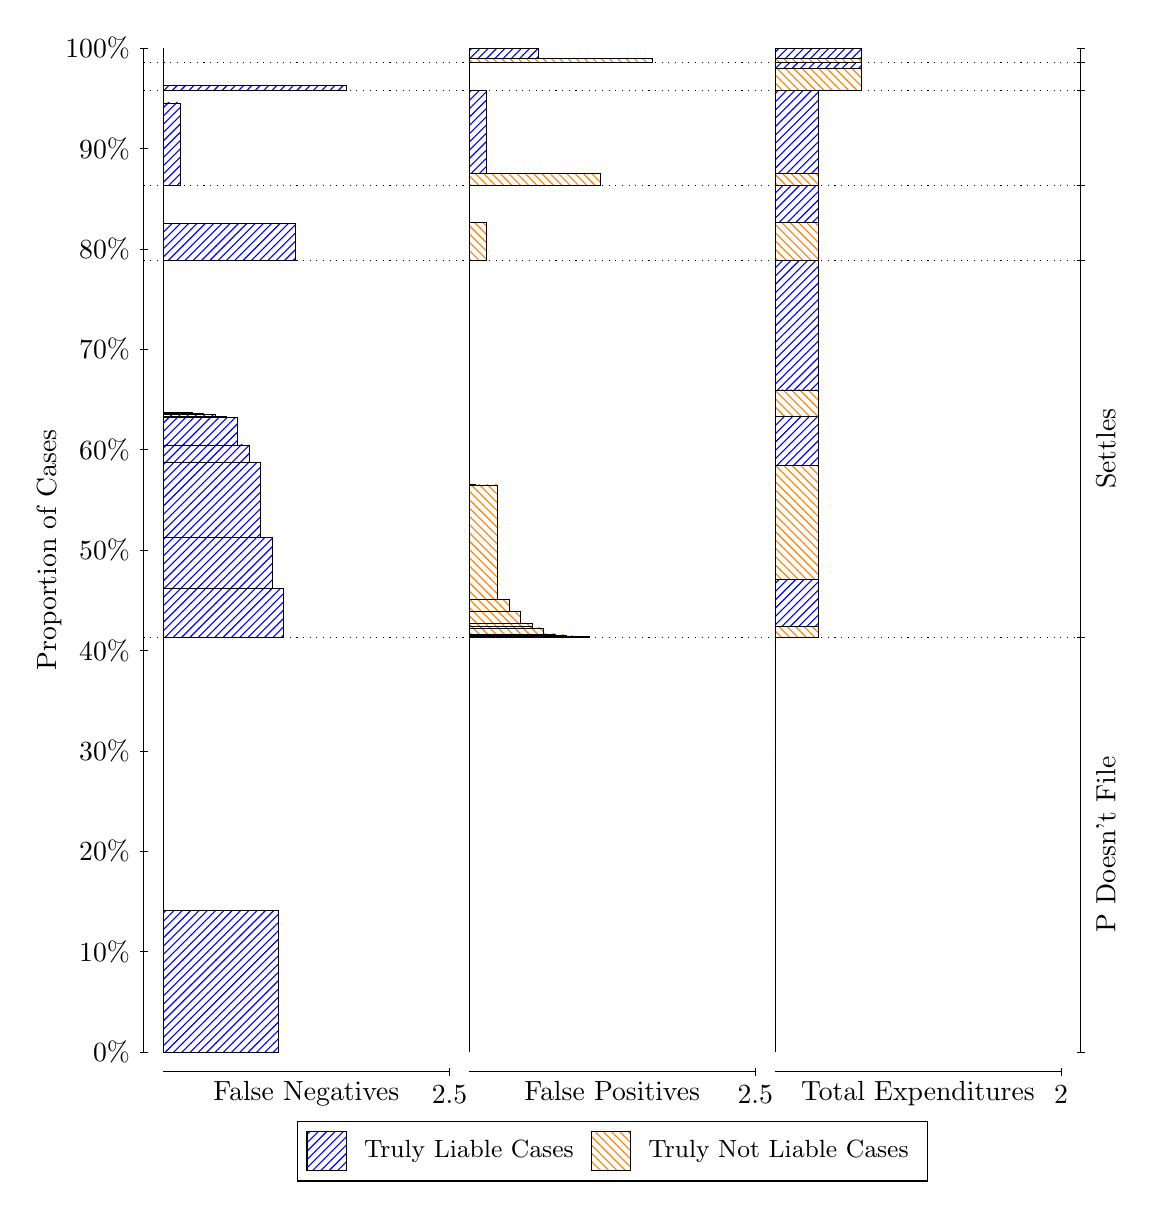
\begin{tikzpicture}
\draw[black, very thin] (1.5,1.75) -- (1.5,14.5);
\node[rotate=90, text=black, anchor=center] at (0.3, 8.125) {Proportion of Cases};
\draw[black, very thin] (1.45,1.75) -- (1.55,1.75);
\node[text=black, anchor=east] at (1.45, 1.75) {0\%};
\draw[black, very thin] (1.45,3.025) -- (1.55,3.025);
\node[text=black, anchor=east] at (1.45, 3.025) {10\%};
\draw[black, very thin] (1.45,4.3) -- (1.55,4.3);
\node[text=black, anchor=east] at (1.45, 4.3) {20\%};
\draw[black, very thin] (1.45,5.575) -- (1.55,5.575);
\node[text=black, anchor=east] at (1.45, 5.575) {30\%};
\draw[black, very thin] (1.45,6.85) -- (1.55,6.85);
\node[text=black, anchor=east] at (1.45, 6.85) {40\%};
\draw[black, very thin] (1.45,8.125) -- (1.55,8.125);
\node[text=black, anchor=east] at (1.45, 8.125) {50\%};
\draw[black, very thin] (1.45,9.4) -- (1.55,9.4);
\node[text=black, anchor=east] at (1.45, 9.4) {60\%};
\draw[black, very thin] (1.45,10.675) -- (1.55,10.675);
\node[text=black, anchor=east] at (1.45, 10.675) {70\%};
\draw[black, very thin] (1.45,11.95) -- (1.55,11.95);
\node[text=black, anchor=east] at (1.45, 11.95) {80\%};
\draw[black, very thin] (1.45,13.225) -- (1.55,13.225);
\node[text=black, anchor=east] at (1.45, 13.225) {90\%};
\draw[black, very thin] (1.45,14.5) -- (1.55,14.5);
\node[text=black, anchor=east] at (1.45, 14.5) {100\%};

\draw[black, very thin] (13.4,1.75) -- (13.4,14.5);
\draw[black, very thin] (13.35,1.75) -- (13.45,1.75);
\node[anchor=west] at (13.35, 1.75) {};
\draw[black, very thin] (13.35,7.0193) -- (13.45,7.0193);
\node[anchor=west] at (13.35, 7.0193) {};
\draw[black, very thin] (13.35,11.801) -- (13.45,11.801);
\node[anchor=west] at (13.35, 11.801) {};
\draw[black, very thin] (13.35,12.752) -- (13.45,12.752);
\node[anchor=west] at (13.35, 12.752) {};
\draw[black, very thin] (13.35,13.959) -- (13.45,13.959);
\node[anchor=west] at (13.35, 13.959) {};
\draw[black, very thin] (13.35,14.313) -- (13.45,14.313);
\node[anchor=west] at (13.35, 14.313) {};
\draw[black, very thin] (13.35,14.5) -- (13.45,14.5);
\node[anchor=west] at (13.35, 14.5) {};

\draw[black, very thin, pattern color=blue, pattern=north east lines] (1.75,1.75) rectangle (3.2033,3.5517);
\draw[black, very thin, pattern color=orange, pattern=north west lines] (1.75,3.5517) rectangle (1.75,7.0193);
\draw[black, very thin, pattern color=blue, pattern=north east lines] (1.75,7.0193) rectangle (3.276,7.6355);
\draw[black, very thin, pattern color=blue, pattern=north east lines] (1.75,7.6355) rectangle (3.1307,8.2891);
\draw[black, very thin, pattern color=blue, pattern=north east lines] (1.75,8.2891) rectangle (2.9853,9.234);
\draw[black, very thin, pattern color=blue, pattern=north east lines] (1.75,9.234) rectangle (2.84,9.46);
\draw[black, very thin, pattern color=blue, pattern=north east lines] (1.75,9.46) rectangle (2.6947,9.8063);
\draw[black, very thin, pattern color=blue, pattern=north east lines] (1.75,9.8063) rectangle (2.5493,9.8263);
\draw[black, very thin, pattern color=blue, pattern=north east lines] (1.75,9.8263) rectangle (2.404,9.8479);
\draw[black, very thin, pattern color=blue, pattern=north east lines] (1.75,9.8479) rectangle (2.2587,9.858);
\draw[black, very thin, pattern color=blue, pattern=north east lines] (1.75,9.858) rectangle (2.1133,9.8695);
\draw[black, very thin, pattern color=orange, pattern=north west lines] (1.75,9.8695) rectangle (1.75,11.801);
\draw[black, very thin, pattern color=blue, pattern=north east lines] (1.75,11.801) rectangle (3.4213,12.271);
\draw[black, very thin, pattern color=orange, pattern=north west lines] (1.75,12.271) rectangle (1.75,12.752);
\draw[black, very thin, pattern color=blue, pattern=north east lines] (1.75,12.752) rectangle (1.968,13.803);
\draw[black, very thin, pattern color=orange, pattern=north west lines] (1.75,13.803) rectangle (1.75,13.959);
\draw[black, very thin, pattern color=blue, pattern=north east lines] (1.75,13.959) rectangle (4.0753,14.027);
\draw[black, very thin, pattern color=orange, pattern=north west lines] (1.75,14.027) rectangle (1.75,14.313);
\draw[black, very thin, pattern color=orange, pattern=north west lines] (1.75,14.313) rectangle (1.75,14.366);
\draw[black, very thin, pattern color=blue, pattern=north east lines] (1.75,14.366) rectangle (1.75,14.5);
\draw[black, very thin, pattern color=orange, pattern=north west lines] (5.6333,1.75) rectangle (5.6333,5.2176);
\draw[black, very thin, pattern color=blue, pattern=north east lines] (5.6333,5.2176) rectangle (5.6333,7.0193);
\draw[black, very thin, pattern color=orange, pattern=north west lines] (5.6333,7.0193) rectangle (7.1593,7.0266);
\draw[black, very thin, pattern color=orange, pattern=north west lines] (5.6333,7.0266) rectangle (7.014,7.0331);
\draw[black, very thin, pattern color=orange, pattern=north west lines] (5.6333,7.0331) rectangle (6.8687,7.0468);
\draw[black, very thin, pattern color=orange, pattern=north west lines] (5.6333,7.0468) rectangle (6.7233,7.06);
\draw[black, very thin, pattern color=orange, pattern=north west lines] (5.6333,7.06) rectangle (6.578,7.1352);
\draw[black, very thin, pattern color=orange, pattern=north west lines] (5.6333,7.1352) rectangle (6.4327,7.1585);
\draw[black, very thin, pattern color=orange, pattern=north west lines] (5.6333,7.1585) rectangle (6.4327,7.1934);
\draw[black, very thin, pattern color=orange, pattern=north west lines] (5.6333,7.1934) rectangle (6.2873,7.3411);
\draw[black, very thin, pattern color=orange, pattern=north west lines] (5.6333,7.3411) rectangle (6.142,7.4975);
\draw[black, very thin, pattern color=orange, pattern=north west lines] (5.6333,7.4975) rectangle (5.9967,8.951);
\draw[black, very thin, pattern color=blue, pattern=north east lines] (5.6333,8.951) rectangle (5.706,8.9625);
\draw[black, very thin, pattern color=blue, pattern=north east lines] (5.6333,8.9625) rectangle (5.6333,11.801);
\draw[black, very thin, pattern color=orange, pattern=north west lines] (5.6333,11.801) rectangle (5.8513,12.282);
\draw[black, very thin, pattern color=blue, pattern=north east lines] (5.6333,12.282) rectangle (5.6333,12.752);
\draw[black, very thin, pattern color=orange, pattern=north west lines] (5.6333,12.752) rectangle (7.3047,12.908);
\draw[black, very thin, pattern color=blue, pattern=north east lines] (5.6333,12.908) rectangle (5.8513,13.959);
\draw[black, very thin, pattern color=orange, pattern=north west lines] (5.6333,13.959) rectangle (5.6333,14.245);
\draw[black, very thin, pattern color=blue, pattern=north east lines] (5.6333,14.245) rectangle (5.6333,14.313);
\draw[black, very thin, pattern color=orange, pattern=north west lines] (5.6333,14.313) rectangle (7.9587,14.366);
\draw[black, very thin, pattern color=blue, pattern=north east lines] (5.6333,14.366) rectangle (6.5053,14.5);
\draw[black, very thin, pattern color=orange, pattern=north west lines] (9.5167,1.75) rectangle (9.5167,5.2176);
\draw[black, very thin, pattern color=blue, pattern=north east lines] (9.5167,5.2176) rectangle (9.5167,7.0193);
\draw[black, very thin, pattern color=orange, pattern=north west lines] (9.5167,7.0193) rectangle (10.062,7.1585);
\draw[black, very thin, pattern color=blue, pattern=north east lines] (9.5167,7.1585) rectangle (10.062,7.7491);
\draw[black, very thin, pattern color=orange, pattern=north west lines] (9.5167,7.7491) rectangle (10.062,9.2027);
\draw[black, very thin, pattern color=blue, pattern=north east lines] (9.5167,9.2027) rectangle (10.062,9.8189);
\draw[black, very thin, pattern color=orange, pattern=north west lines] (9.5167,9.8189) rectangle (10.062,10.158);
\draw[black, very thin, pattern color=blue, pattern=north east lines] (9.5167,10.158) rectangle (10.062,11.801);
\draw[black, very thin, pattern color=orange, pattern=north west lines] (9.5167,11.801) rectangle (10.062,12.282);
\draw[black, very thin, pattern color=blue, pattern=north east lines] (9.5167,12.282) rectangle (10.062,12.752);
\draw[black, very thin, pattern color=orange, pattern=north west lines] (9.5167,12.752) rectangle (10.062,12.908);
\draw[black, very thin, pattern color=blue, pattern=north east lines] (9.5167,12.908) rectangle (10.062,13.959);
\draw[black, very thin, pattern color=orange, pattern=north west lines] (9.5167,13.959) rectangle (10.607,14.245);
\draw[black, very thin, pattern color=blue, pattern=north east lines] (9.5167,14.245) rectangle (10.607,14.313);
\draw[black, very thin, pattern color=orange, pattern=north west lines] (9.5167,14.313) rectangle (10.607,14.366);
\draw[black, very thin, pattern color=blue, pattern=north east lines] (9.5167,14.366) rectangle (10.607,14.5);
\draw[black, dotted] (1.5,7.0193) -- (13.4,7.0193);
\draw[black, dotted] (1.5,11.801) -- (13.4,11.801);
\draw[black, dotted] (1.5,12.752) -- (13.4,12.752);
\draw[black, dotted] (1.5,13.959) -- (13.4,13.959);
\draw[black, dotted] (1.5,14.313) -- (13.4,14.313);
\draw[black, very thin] (1.75,1.5) -- (5.3833,1.5);
\node[text=black, anchor=north] at (3.5667, 1.5) {False Negatives};
\draw[black, very thin] (5.3833,1.45) -- (5.3833,1.55);
\node[text=black, anchor=north] at (5.3833, 1.45) {2.5};

\draw[black, very thin] (5.6333,1.5) -- (9.2667,1.5);
\node[text=black, anchor=north] at (7.45, 1.5) {False Positives};
\draw[black, very thin] (9.2667,1.45) -- (9.2667,1.55);
\node[text=black, anchor=north] at (9.2667, 1.45) {2.5};

\draw[black, very thin] (9.5167,1.5) -- (13.15,1.5);
\node[text=black, anchor=north] at (11.333, 1.5) {Total Expenditures};
\draw[black, very thin] (13.15,1.45) -- (13.15,1.55);
\node[text=black, anchor=north] at (13.15, 1.45) {2};

\node[text=black, centered, rotate=90] at (13.72, 4.3846) {P Doesn't File};
\node[text=black, centered, rotate=90] at (13.72, 9.4103) {Settles};





\draw (7.449999999999999,1.5) node[draw=none] (baseCoordinate) {};
\begin{scope}[align=center]
        \matrix[scale=0.5, draw=black, below=0.5cm of baseCoordinate, nodes={draw}, column sep=0.1cm]{
            \node[rectangle, draw, minimum width=0.5cm, minimum height=0.5cm, pattern color=blue, pattern=north east lines] {}; &
            \node[draw=none, font=\small, text=black] (B) {Truly Liable Cases}; &
            \node[rectangle, draw, minimum width=0.5cm, minimum height=0.5cm, pattern color=orange, pattern=north west lines] {}; &
            \node[draw=none, font=\small, text=black] (B) {Truly Not Liable Cases}; \\
            };
\end{scope}

\end{tikzpicture}
\end{document}